\begin{steps}[leftmargin=*]
    % \item Read the document once.
    % If you have issues understanding something we encourage you to ask the supervisor or look up any terms/companies/acronyms.
    
    \item \label{step:start} Read the \textbf{next sentence}.
    If \eventcolor \texttt{a\_Event} annotations already exist: go to step \ref{step:forevent}
    If no pre-existing \texttt{a\_Event} are present: go to step \ref{step:annotatesentiment}
    
    \item \label{step:forevent} Decide \hyperlink{sec:polaritydefinition}{\textbf{Polarity}} for each \hyperlink{sec:eventdefinition}{pre-existing \texttt{a\_Event}}.
    \begin{enumerate}[label=\alph*), leftmargin=*] \label{step:polarity}% insert figure here and explain in more detail
        \item \texttt{Positive}: the event/sentiment is mostly positive.
        \item \texttt{Negative}: the event/sentiment is mostly negative.
        \item \texttt{Neutral}: the event/sentiment has no clear positive or negative connotation.
        \item \texttt{Conflict}: the event/sentiment depends on the point-of-view.
    \end{enumerate}
    \textcolor{OliveGreen}{Click on each \eventcolor \texttt{a\_Event} annotation and choose Polarity using the \texttt{i\_Polarity} drop-down menu in the side panel.}
    
    \item \label{step:annotatesentiment} Annotate all \hyperlink{sec:sentimentexpressiondefinition}{\textbf{Sentiment Expressions}} as the \textbf{smallest possible number of words} denoting \hyperlink{sec:sentimentdef}{investor sentiment} in the sentence. % 
    \textit{Which words express an opinion or could affect an investors opinion?}\\
    \textcolor{OliveGreen}{Select \texttt{1\_Sentiment} in the Layer drop-down menu (top-right side panel), drag the mouse across the words that express the sentiment in the Annotation panel. \footnotesize{Selection of the annotation layer fails sometimes. To fix: Unselect the current annotation with the \texttt{Clear} button, select a different layer than \texttt{1\_Sentiment} and next re-select \texttt{1\_Sentiment}.}}\\
    \textcolor{BrickRed}{NOTE: Sentiment words that are part of/overlap with a pre-existing Event/Entity but do not correspond fully in meaning $\rightarrow$ Annotate a new overlapping Sentiment Expression.}\\
    % NOTE: Sentiment words overlap with existing event: If the sentiment words intensify or change the opinion of the smaller event annotation, annotate the sentiment expression separately including the event words so that they overlap.
    
    
    \item \label{step:decidetargets} Select each \texttt{1\_Sentiment} and annotate all the \hyperlink{sec:targetdefinition}{\textbf{Targets}}.
    \textit{What is the opinion about?}.\\
    One Sentiment Expression can have \textbf{multiple targets}: make sure links are drawn to each target.\\
    \textcolor{OliveGreen}{While the \sentimentcolor \texttt{1\_Sentiment} annotation is selected (glowing outline)}:
        \begin{enumerate}[label=\alph*), leftmargin=*]
            \item \label{step:linkentity} Target is \hyperlink{sec:entitydefinition}{a pre-existing \entitycolor Entity} $\rightarrow$ \textbf{Link Entity}:\\
            \textcolor{OliveGreen}{
            Click on the \texttt{Click to activate} field next to ``EntityIsTarget'' in the side panel.
            Click on the \entitycolor \texttt{b\_Entity} in the Annotation panel.
            }
            \item \label{step:linkevent} Target is \hyperlink{sec:eventdefinition}{a pre-existing \eventcolor Event} $\rightarrow$ \textbf{Link Event}:\\
            \textcolor{OliveGreen}{
            Click on the \texttt{Click to activate} field next to "EventIsTarget" in the side panel.
            Click on the \eventcolor \texttt{a\_Event} in the Annotation panel.
            }
            \item \label{step:newtarget} Target on words without an existing annotation $\rightarrow$ \textbf{Create and Link a new target}:\\
            \textcolor{OliveGreen}{
            Click on the \texttt{Click to activate} field next to "EventIsTarget" in the side panel.
            Drag your mouse across the smallest possible amount of words indicating the entity in the Annotation panel.
            }
            \item \label{step:multiple} Multiple targets $\rightarrow$ \textbf{Add more than one target}:\\
            \textcolor{OliveGreen}{
            Click on \texttt{Select Role} in the drop-down menu under ``EntityIsTarget'' (if target is existing or new Entity) or ``EventIsTarget'' (if target is existing Event) and click the \texttt{Add} button. Proceed as in the previous options.
            }
        \end{enumerate}
        
        \item Decide \hyperlink{sec:polaritydefinition}{\textbf{Polarity}}, cf. step \ref{step:polarity}.\\
        \textcolor{BrickRed}{NOTE: Sometimes the sentiment polarity is different depending on the target. In these cases, we make a new sentiment annotation and link Targets to which the sentiment polarity corresponds.}
        
        \item Decide \hyperlink{sec:uncertaintydefinition}{\textbf{Uncertainty}}: \textit{Is the sentiment expression presented as being uncertain?}\\
        \textcolor{OliveGreen}{
        Toggle \texttt{d\_Uncertain} from red ``No'' to green ``Yes'' in the side panel.
        }
        
        \item Decide \hyperlink{sec:negationdefinition}\textbf{Negation}: \textit{Is the sentiment expression negated?}\\
        \textcolor{OliveGreen}{
        Toggle \texttt{e\_Negated} from red ``No'' to green ``Yes'' in the side panel.
        }
        
    \item Continue on to the next sentence; go to step \ref{step:start}
    
\end{steps}

\begin{figure}[!htb]
    \centering
    \caption*{Workflow overview chart}
    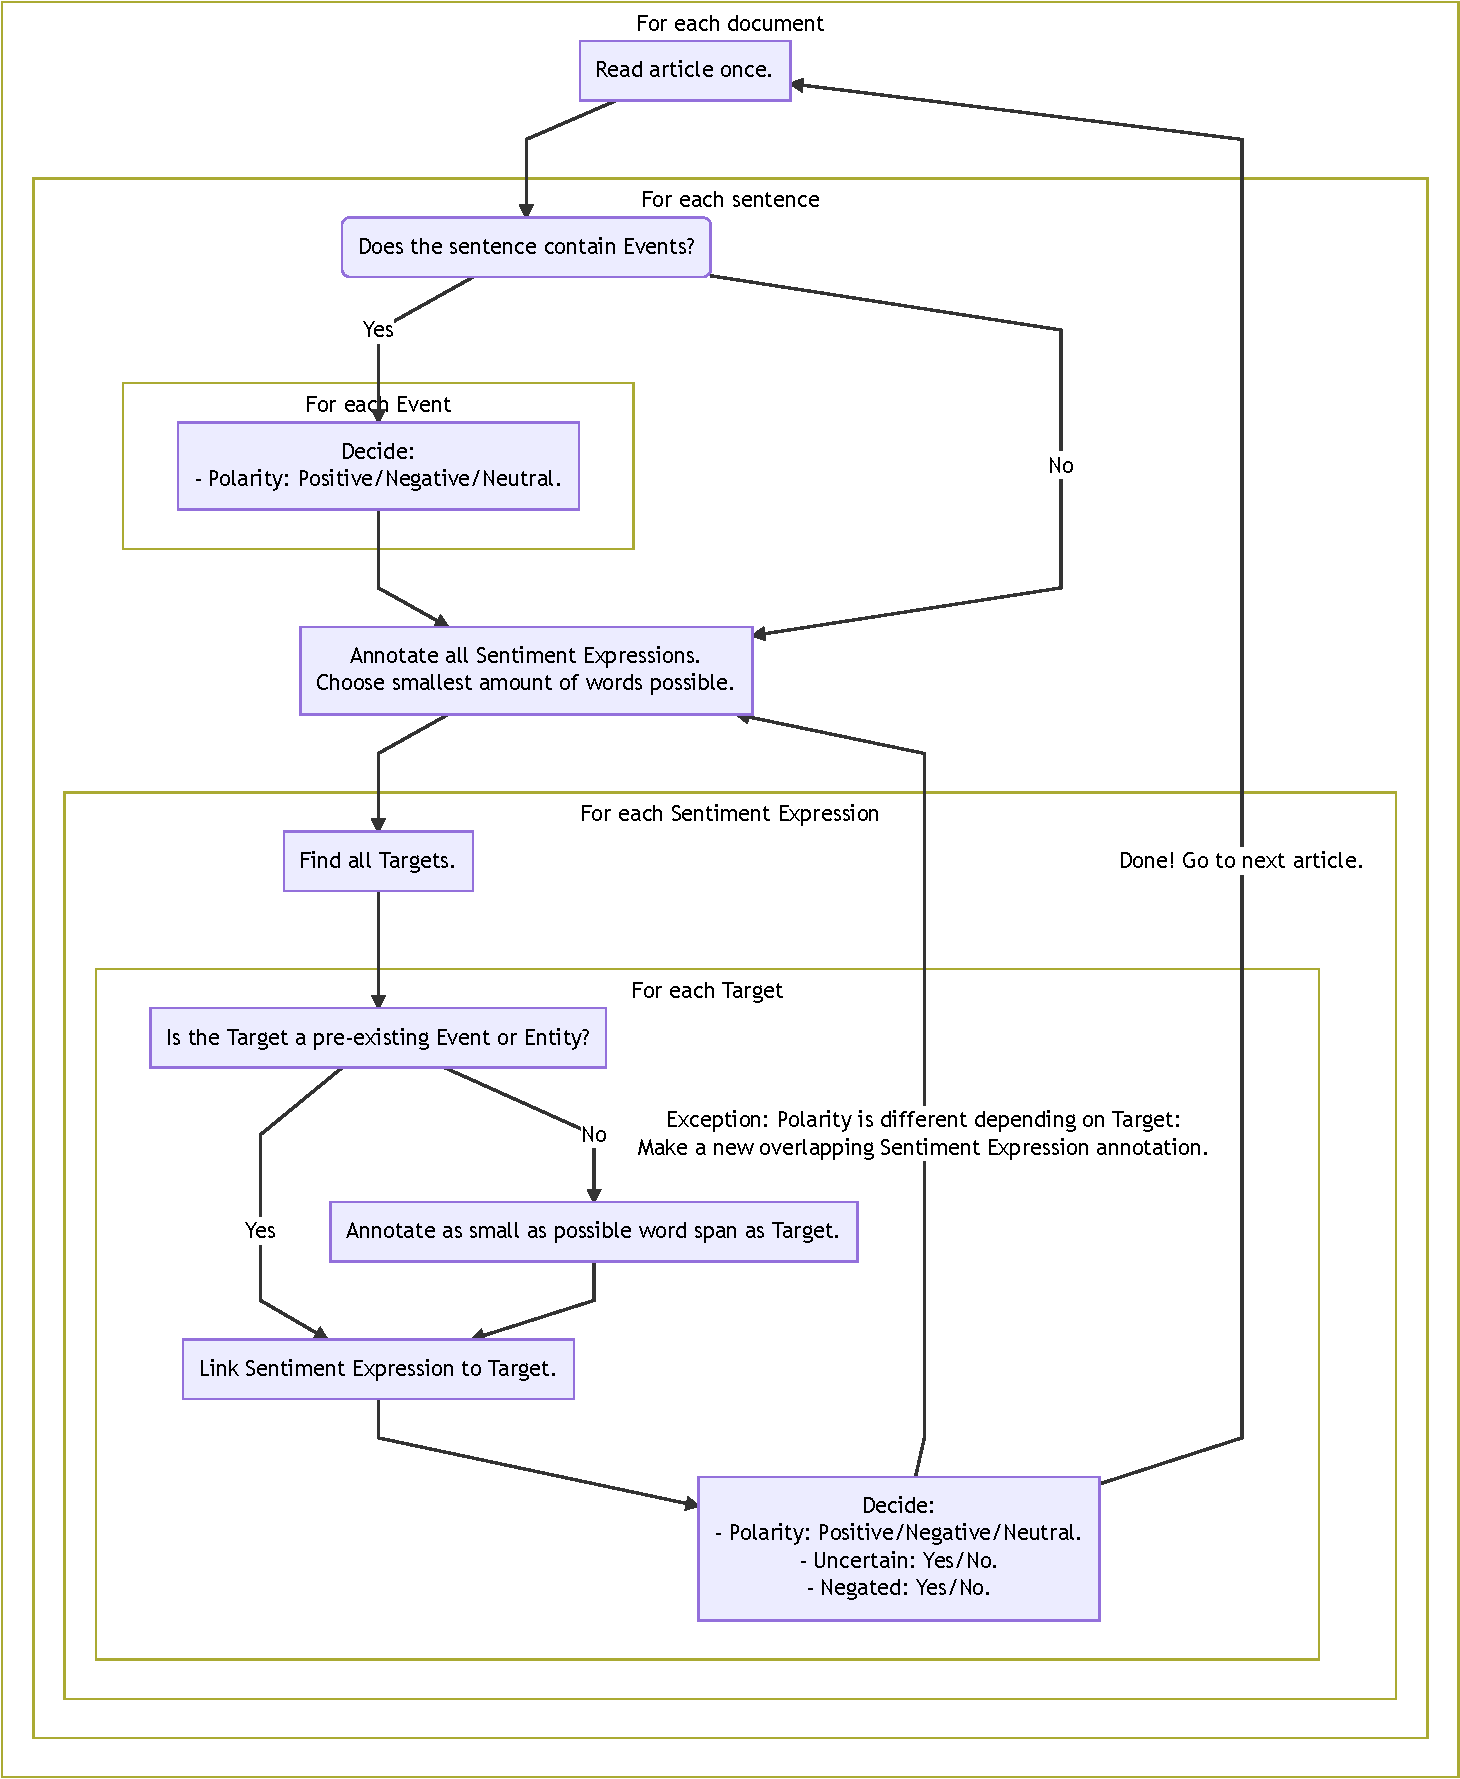
\includegraphics[width=\textwidth]{img/workflow-diagram-cropped.pdf}
\end{figure}